\chapter{Simulace ve virtuálním prostředí}

Simulátory umožňují letovému kódu PX4 ovládat počítačem namodelovaný dron\break v simulovaném \uv{světě}. S tímto dronem je možné komunikovat stejně jako se skutečným dronem pomocí software QGroundControl, \textit{offboard} API nebo rádiového ovladače/gamepadu. 

PX4 podporuje jak simulaci \acs{SITL} (\textit{\acl{SITL}}), kde PX4 firmware (program řídící jednotky) běží na počítači, nebo simulaci \acs{HITL} (\textit{\acl{HITL}}), kde PX4 firmware běží na skutečné řídící jednotce a vše ostatní (fyzika reálného světa) je spuštěno na počítači. \cite{PX4docs}

Všechny simulátory mohou komunikovat s firmware PX4 pomocí \textit{Simulator MAVLink API}, které definuje sadu zpráv MAVLink. Na obrázku \ref{fig:SIM1} je zobrazen tok zpráv mezi \uv{simulovaným světem} a mezi firmware PX4.

\begin{figure}[!ht]
  \begin{center}
    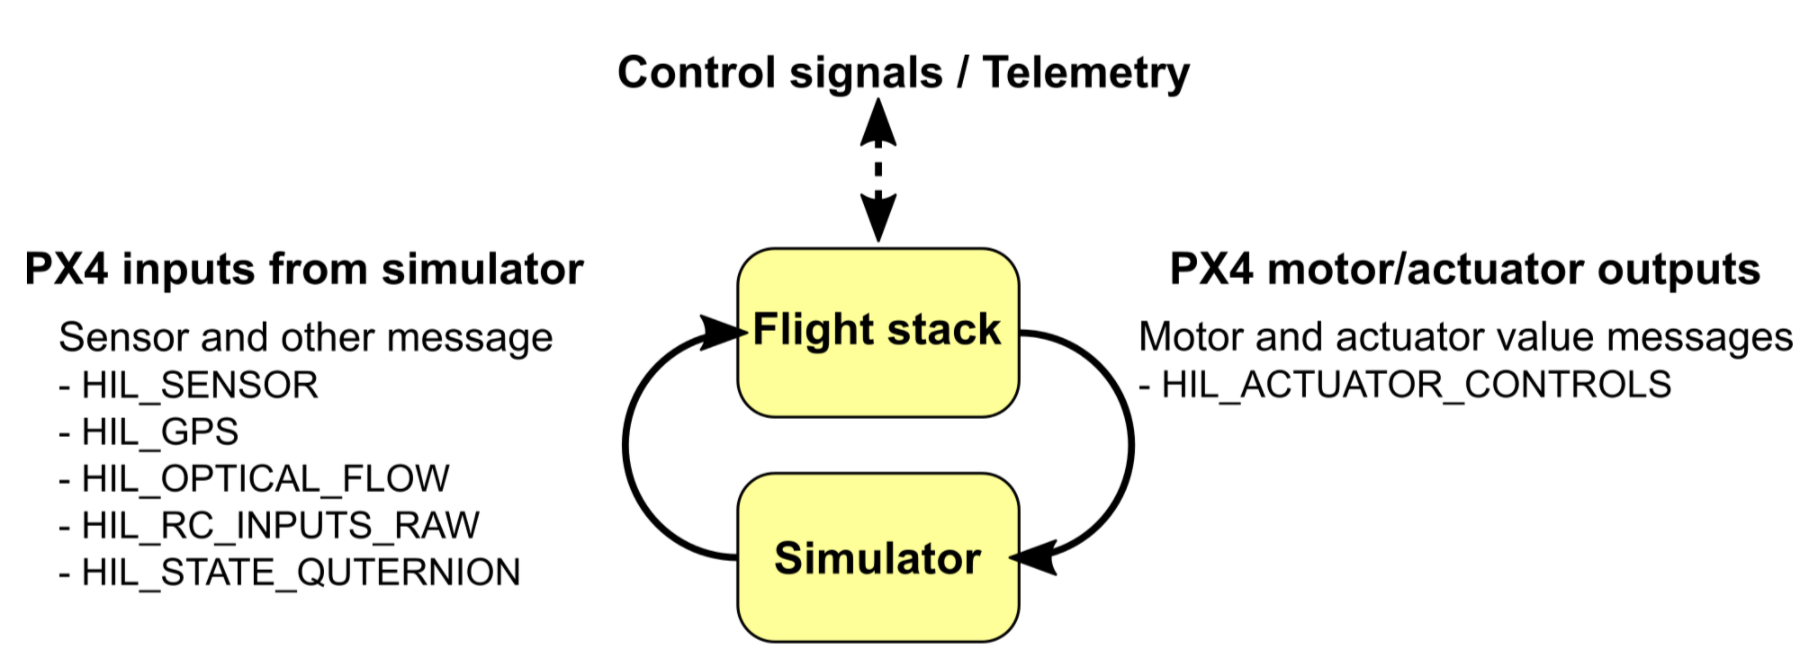
\includegraphics[scale=0.3]{obrazky/SIM1}
  \end{center}
  \caption[Tok zpráv mezi simulátorem a PX4]{Tok zpráv mezi simulátorem a PX4 \cite{PX4docs}.}
  \label{fig:SIM1}
\end{figure}

\section{SITL simulační prostředí}

\textit{\acl{SITL}} simulace umožňuje rychlé a \uv{levné} ladění robotických misí, protože pro simulaci \acs{SITL} se nevyužívá žádný specializovaný hardware, ale jenom počítač s nainstalovaným simulačním prostředím.

Obrázek \ref{fig:SIM2} zobrazuje typickou konfiguraci simulace \acs{SITL} pro PX4 firmware\break a pro kterýkoliv z podporovaných simulátorů. Simulátor a PX4 firmawe mohou spolu komunikovat pomocí MAVLink \acs{API}. Pro přímou interakci s PX4 je možné využít komunikaci přes \textit{Micro-RTPS bridge}, kde se komunikují přímo uORB zprávy.

Různé části simulačního prostředí spolu komunikují pomocí \acs{UDP} (\acl{UDP}) a mohou být spuštěny na stejném počítači, nebo jiném počítači ve stejné síti. Pomocí sériové komunikace je možné připojit joystick, gamepad nebo RC soupravu pro ruční ovládání simulovaného dronu přes QGroundControl.

\begin{figure}[!ht]
  \begin{center}
    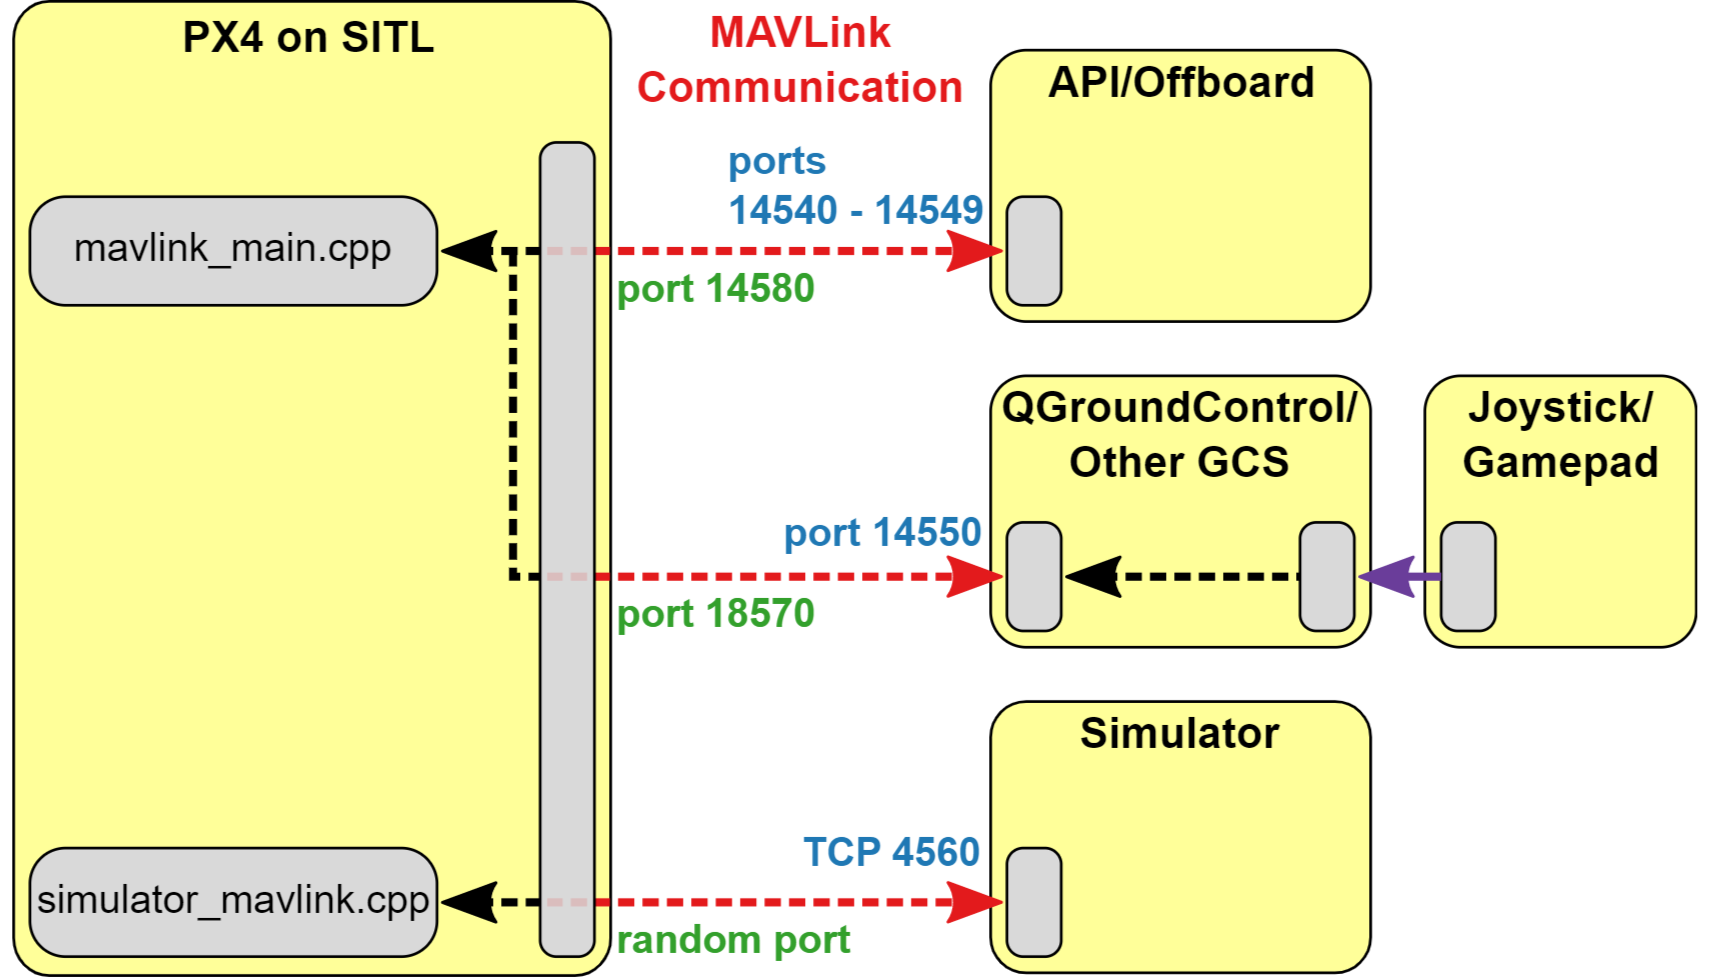
\includegraphics[scale=0.32]{obrazky/SIM2}
  \end{center}
  \caption[Schéma komunikace mezi PX4 a simulátorem]{Schéma komunikace mezi PX4 a simulátorem \cite{PX4docs}.}
  \label{fig:SIM2}
\end{figure}

\subsection{Seznam podporovaných simulátorů}

Následující simulátory jsou podporovány systémem PX4:

\begin{itemize}
    \item Gazebo
    \item FlightGear
    \item JSBSim
    \item jMAVSim
    \item AirSim
    \item Ignition Gazebo
\end{itemize}

\subsection{Gazebo}

Simulátor Gazebo je vysoce doporučen pro PX4 \textit{\acl{SITL}} simulaci.

Gazebo je dobře navržený a otestovaný simulátor, umožňující rychlé testování algoritmů, návrh robotů a trénování systémů s umělou inteligencí v realistických scénářích. Nabízí možnost přesně a efektivně simulovat populace robotů ve složitých vnitřních i venkovních prostředích. Gazebo se běžně používá pro práci s ROS (ROS 2).  \cite{ROSROBOT}

Podporovaná vozidla \acs{SITL} simulace PX4 v simulátoru Gazebo jsou: \cite{GAZ}

\begin{itemize}
    \item dron
    \item delta \acs{VTOL} (\acl{VTOL})
    \item letadlo
    \item rover
    \item ponorka
\end{itemize}

\subsection{Ignition Gazebo}

Vývojový tým simulátoru Gazebo se v budoucnu zaměří na vývoj simulátoru Ignition, takže Gazebo 11 je poslední verze známého simulátoru Gazebo. Oba simulátory jsou kompatibilní ve formátu popisu prostředí (\uv{světa}) a některých pluginů. \cite{IGN}

Z důvodu, že simulační firmware PX4 je v této době lépe přepojený se simulátorem Gazebo, tak v této práci budeme pracovat s simulátorem Gazebo 11.

Jediné vozidlo, které je podporované \textit{\acl{SITL}} simulací PX4 v simulátoru Ignition, je dron.

\section{Instalace virtuálního prostředí}

Pro vývoj a simulaci bezpilotních misí v prostředí PX4 a ROS 2 je nutné nainstalovat jednotlivé komponenty vývojového prostředí:

\begin{itemize}
    \item PX4 simulační firmware
    \item Gazebo simulátor
    \item ROS 2 
    \item Komunikační most mezi PX4 firmware a ROS 2
    \begin{itemize}
        \item PX4 - ROS 2 \textit{bridge}
        \item Mavros\\
    \end{itemize}
\end{itemize}

V následujících podkapitolách si popíšeme instalaci jednotlivých částí. Návod je určený pro linuxovou distribuci Ubuntu 20.04 \textit{Focal Fossa}.

\subsection{Instalace PX4 simulačního prostředí}

Prvním krokem je instalace PX4 prostředí. Při reální misi (nebo \acs{HITL} simulaci) bude PX4 firmware spuštěný přímo na řídící jednotce Pixhawk. Při \acs{SITL} simulaci je nutné PX4 letový kód nainstalovat na počítač. Doporučená platforma pro PX4 prostředí je Ubuntu, ale je možné ho spustit na Windows 10 nebo na Mac OS.

Samotná instalace prostředí PX4 je jednoduchá a skládá se z dvou kroků. \cite{PX4docs}

\begin{lstlisting}[language=bash]
# 1. Stáhnout zdrojový kód PX4:
$ git clone https://github.com/PX4/PX4-Autopilot.git --recursive
 
# 2. Spustit script ubuntu.sh bez argumentů
# pro instalaci všech závislostí
$ bash ./PX4-Autopilot/Tools/setup/ubuntu.sh
\end{lstlisting}

Script \texttt{ubuntu.sh} nastaví vývojové prostředí PX4, dále nainstaluje simulátory Gazebo a jMavSim a sadu nástrojů \textit{NuttX}\footnote{NuttX je \acs{RTOS} (\acl{RTOS}) pro provoz PX4 na řídící jednotce Pixhawk. Je to open source (BSD licence), lehký, výkonný a velmi stabilní operační systém. \cite{PX4docs}}/\textit{Pixhawk}

\subsection{Instalace ROS 2 Foxy a všech závislostí}

Instalace ROS 2 je dobře popsaná na dokumentačních stránkách \cite{ROS2INSTALL}. Po úspěšné instalaci ROS 2 Foxy je nutné doinstalovat několik závislostí:

\begin{lstlisting}[language=bash]
# 1. Instalační proces ROS 2 by měl nainstalovat 
#    nástroje pro sestavení colcon, ale v případě, 
#    že se tak nestane, můžete nástroje nainstalovat ručně:
$ sudo apt install python3-colcon-common-extensions
 
# 2. Eigen3 se používá v knihovně transformací:
$ sudo apt install ros-foxy-eigen3-cmake-module
 
# 3. Další závislosti Pythonu musí být také nainstalovány:
$ sudo pip3 install -U empy pyros-genmsg 
$ pip3 install transforms3d

# 3. Nainstalovat pluginy do simulátoru gazebo:
$ sudo apt install ros-foxy-gazebo-ros-pkgs
\end{lstlisting}

\subsection{Komunikace pomocí \acs{RTPS}}

Jak je popsáno v kapitole \ref{sec:komunikace} \nameref{sec:komunikace}, pro komunikaci mezi ROS 2 \textit{node} a PX4 slouží \textit{eProsima Fast DDS}, který umožňuje výměnu zpráv uORB mezi PX4 a ROS 2.\\

Pro nastavení PX4 - ROS 2 \textit{bridge} potřebujeme nainstalovat následující balíčky:

\begin{itemize}
    \item Java JDK (Open source JDK 11)
    \item Gradle
    \item Fast-RTPS-Gen\\
\end{itemize}

Po úspěšné instalaci  balíčků je nutné sestavit ROS 2 workspace.

\subsubsection{Java JDK}

Java JDK je nutná závislost pro správné sestavení komunikačního RTPS agenta.

\begin{lstlisting}[language=bash]
$ sudo apt install openjdk-11-jdk
\end{lstlisting}

\subsubsection{Gradle}

Gradle je univerzální nástroj pro sestavení software v jazycích C++, Swift, Java.\break V našem případě je nutný pro sestavení komunikačního \acs{RTPS} agenta.

Gradle je možné nainstalovat pomocí následujících příkazů \cite{GRADLE}:

\begin{lstlisting}[language=bash]
# Stažení, extrahování a vytvoření odkazu
$ wget https://services.gradle.org/distributions/gradle-6.3-bin.zip \
  -P /tmp
$ sudo unzip -d /opt/gradle /tmp/gradle-6.3-bin.zip
$ sudo ln -s /opt/gradle/gradle-6.3 /opt/gradle/latest
\end{lstlisting}

Pro přidání Gradle adresářu do systémové proměnné \texttt{PATH} je nutné vytvořit soubor \texttt{/etc/profile.d/gradle.sh} a přidat následnou konfiguraci.

\begin{lstlisting}[language=bash]
$ sudo nano /etc/profile.d/gradle.sh
\end{lstlisting}

\begin{lstlisting}[language=bash]
  export GRADLE_HOME=/opt/gradle/latest
  export PATH=${GRADLE_HOME}/bin:${PATH}
\end{lstlisting}

Následně je nutné změnit oprávnění skriptu pomocí příkazu:

\begin{lstlisting}[language=bash]
$ sudo chmod +x /etc/profile.d/gradle.sh
\end{lstlisting}

\subsubsection{Fast RTPS Gen}

Fast-RTPS-Gen je nástroj pro generování \acs{IDL} (\acl{IDL}) kódu pro Fast RTPS (\acs{DDS}).

Fast-RTPS-Gen je možné nainstalovat pomocí následujících příkazů:

\begin{lstlisting}[language=bash]
# Načtení proměnných prostředí
$ source /etc/profile.d/gradle.sh

# Stažení a sestavení Fast DDS Generátoru
$ git clone https://github.com/eProsima/Fast-DDS-Gen.git \
  --recursive -b v1.0.4 ~/Fast-RTPS-Gen \
  && cd ~/Fast-RTPS-Gen \
  && gradle assemble \
  && sudo env "PATH=$PATH" gradle install
\end{lstlisting}

\subsubsection{Sestavení ROS 2 pracovního prostoru}

Pro vytvoření ROS 2 pracovního prostoru (\textit{workspace}) podporujícího simulaci v PX4 s komunikací pomocí \acs{RTPS} je nutné stáhnout dva ROS 2 balíčky. \cite{PX4docs}

Na stáhnutí a sestavení obou balíčků můžeme použít tyto příkazy:

\begin{lstlisting}[language=bash]
# Naklonování obou balíčků:
$ mkdir -p ~/px4_ros_missions/src
$ git clone https://github.com/PX4/px4_ros_com.git \
  ~/px4_ros_missions/src/px4_ros_com
$ git clone https://github.com/PX4/px4_msgs.git \
  ~/px4_ros_missions/src/px4_msgs
  
# Balíček px4_ros_com obsahuje scripty na sestavení workspace:
$ cd ~/px4_ros_missions/src/px4_ros_com/scripts
$ source build_ros2_workspace.bash
\end{lstlisting}

\subsubsection{Balíček \texttt{px4\_msgs}}

V balíčku \texttt{px4\_msgs} je nadefinovaných víc jak 200 uORB zpráv pro komunikaci mezi ROS 2 \textit{node} a PX4 firmware.

\subsubsection{Balíček \texttt{px4\_ros\_com}}

Balíček \texttt{px4\_ros\_com} generuje přepojení (\textit{MicroRTPS\_agent}) mezi ROS 2 a PX4 firmware pomocí Fast RTPS (\acs{DDS}).\\

\acs{RTPS} agent se na palubním počítači spouští pomocí příkazu:

\begin{lstlisting}[language=bash]
$ source ~/px4_ros_missions/install/setup.bash
$ micrortps_agent -t UDP
\end{lstlisting}

\subsection{Komunikace pomocí MAVLink}

Pro komunikaci ROS 2 s autopilotem PX4 pomocí protokolu MAVLink je nutné nainstalovat ROS 2 balíček Mavros.

Pro instalaci balíčku Mavros slouží následující příkaz:

\begin{lstlisting}[language=bash]
$ sudo apt install ros-foxy-mavros
\end{lstlisting}

Pro správnou funkci balíčku Mavros je nutné doinstalovat geografický dataset (\texttt{geographiclib dataset}), který slouží na převod mezi zeměpisnými, UTM, UPS, MGRS, geocentrickými a místními kartézskými souřadnicemi, pro výpočty gravitace, výšky geoidu a geomagnetického pole a pro řešení geodetických úloh. \cite{GEOLIB}

K tomu slouží následující příkazy:

\begin{lstlisting}[language=bash]
$ wget https://raw.githubusercontent.com/mavlink/mavros\
  /ros2/mavros/scripts/install_geographiclib_datasets.sh
$ sudo bash install_geographiclib_datasets.sh
$ rm install_geographiclib_datasets.sh

# Nainstalování python závislosti:
$ sudo apt install python3-lxml libxml2-utils
\end{lstlisting}
